\chapter{Certificaatautoriteiten}
\label{ch:certificaatautoriteiten}

Certificaatautoriteiten bestaan als externe betrouwbare partij om te bewijzen
dat een entiteit en een publieke sleutel aan elkaar gelinkt zijn. Een voorbeeld
hiervan zijn https-certificaten. Deze bevatten onder andere een domeinnaam, een
publieke sleutel en een digitale handtekening van de certificaatautoriteit. Als
een browser verbindt met een server, stuurt deze server een certificaat door
waarna de browser controleert of de domeinnaam op het certificaat overeenkomt
met de site die bezocht wordt en of het certificaat is ondertekend door een
certificaatautoriteit die vertrouwd wordt. Als deze validatie succesvol is, dan
zal de verdere communicatie met de server geëncrypteerd worden met de publieke
sleutel op het certificaat.

\begin{figure}[H]
	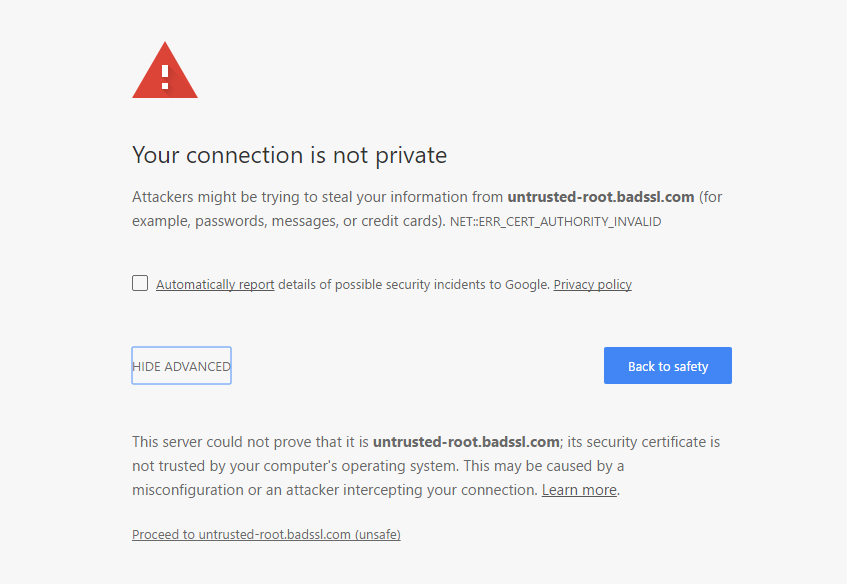
\includegraphics[width=\textwidth,height=\textheight,keepaspectratio]{img/untrusted-root-chrome.png}
	\centering
	\caption{Waarschuwing wanneer een certificaat niet door een certificaat
		authoriteit wordt vertrouwd op Chrome 57.0.2987}
	\label{fig:untrusted-root-chrome}
\end{figure}

\section{Problemen met certificaatautoriteiten}
\label{sec:problemen-met-certificaatautoriteiten}

Het gehele systeem van een vertrouwde derde partij staat en valt bij het juiste
handelen van deze partij. Van elke CA wordt verwacht dat zij enkel certificaten
uitreiken aan de geverifieerde eigenaar van een entiteit. Wanneer een CA een
certificaat uitreikt dan zal dit certificaat vertrouwd worden ongeacht de
toestemming van de eigenaar van de entiteit.

Gevallen van onrechtmatige uitgave van certificaten komen voor en worden actief
gebruikt. In augustus 2011 werd vastgesteld dat een CA in Nederland, DigiNotar,
slachtoffer was geworden van een hack waarbij alle acht signing servers waren
gecompromitteerd. Er waren certificaten voor *.google.com gemaakt alsook
certificaten voor Yahoo, Mozilla, WordPress en The Tor Project. In totaal werden
er meer dan 500 certificaten gegenereerd. Het primaire doel van de aanval was
300 000 Iraanse Gmail gebruikers. De Iraanse regering wordt verdacht van het
uitvoeren van de hack. De NSA, de militaire intelligentie organisatie van de
Verenigde Staten, wordt ook verdacht van het inbreken in DigiNotar en het
ongeoorloofd aanmaken van certificaten \autocite{DiginotarNu,
	DigiNotarThreatpost, DigiNotarComputerworld, DigiNotarSchneier,
	DigiNotarTweakers}.

Op 25 juni 2014 gaf een CA in India certificaten uit voor 45 Google domeinen
waarna deze op de 2de juli werden ontdekt. Google heeft bijgevolg het volledig
vertrouwen in de certificaat autoriteiten opgezegd \autocite{Wilson2014}.

Verder onregelmatigheden gebeurden met de WoSign CA die certificaten aanmaakte
met de verkeerde uitgavedatums om de restrictie op SHA1 te ontlopen. WoSign
kocht ook een andere CA op zonder dit publiek te maken. Een combinatie met
andere gevallen van wangedrag leidde tot het stoppen van het vertrouwen in beide
CAs waarin oude certificaten nog beperkt geldig zullen zijn. Het vertrouwen in
beide CAs wordt volledig uitgefaseerd  \autocite{WoSignMozilla, WoSignTweakers1,
	WoSignTweakers2}.
